\section{Conclusions}

We have developed equivalence theory, the approach used in most lattice physics codes to estimate cross sections in the resonance region of the spectrum for reactor calculations.

Despite being popular and widely used, equivalence theory has several deficiencies. For example, it does not account for resonance overlap (this can be significant for Sm149 and U238, for example), nor does it account for inelastic scattering (which is very significant in fast reactor physics and leads to significant energy loss). These can be accounted for with semi-empirical means (like resonance interference tables) or by more sophisticated (and more expensive) approaches.

There are several alternatives to equivalence theory: at the extreme end, the full slowing down equation could be solved in many groups and is done increasingly commonly, but this can be extremely slow. Likewise, it is common to simply generate cross sections via Monte Carlo -- while also slow, this is easier to implement and use than a lattice physics code and exactly treats geometry. These approaches tend not to be necessary unless the spectrum is fast (e.g., the common use case for ECCO), there is significant burn-up occurring or, for Monte Carlo in particular, the geometry deviates significantly from a large LWR.

There are several important topics which have not been covered in these lectures which are also very important for cross section generation. One is scattering anisotropy: we typically perform transport simulations approximating scattering as isotropic -- but this is not the case. The way around this is to perform a `transport correction', accounting for the (mainly hydrogen-induced) linear anisotropy by having neutrons fly further before colliding (reducing the total cross section) while retaining an isotropic scattering kernel. Choosing how to do this correction is a subject of some interest, although there seems to be increasing concensus about how best to do it for LWRs at least. Another important topic is leakage correction: lattice physics works by assuming that the spectra of pins and assemblies are essentially only determined by their local surroundings, and not their position within the reactor core. This is done by imposing reflective boundaries, i.e., there is no net leakage from an assembly. In a real reactor, there is of course net leakage from certain assemblies to their neighbours (giving the cosine/Bessel shape) or even strongly dissimilar neighbours, which will induce a change in the spectrum from the reflected system. There are techniques to account for this in the generation of cross sections also.
\vspace{10pt}
\begin{figure}[h]
  \centering
  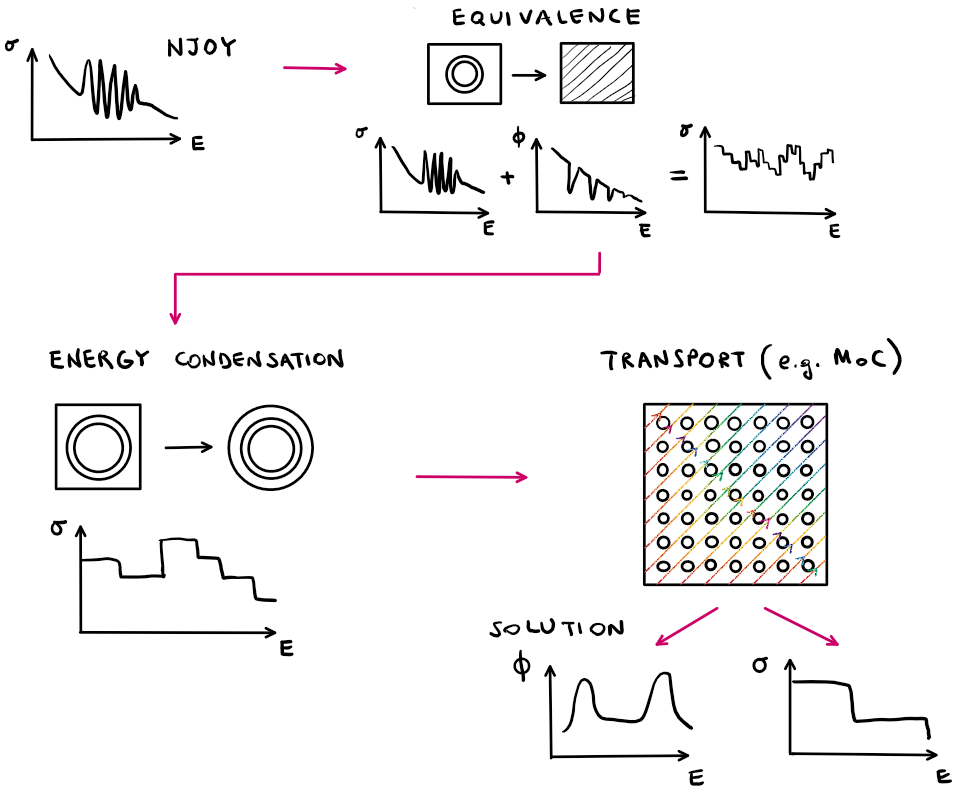
\includegraphics[width=\textwidth]{./Figures/P7/summary_lattice_physics.png} 
  \caption{The usual flow of modern LWR lattice physics codes. NJOY provides processed nuclear data. Equivalence theory is applied to all pin cells to produce self-shielded cross sections in the library fine multigroup structure. Energy condensation is performed at a pin cell level using a collision probabilities solver. Assembly-level transport is performed using a transport solver, producing cross sections for a nodal code, or producing the final solution in some cases.} 
  \label{fig:lattice}
\end{figure}

Following such calculations, what next? This is shown in Fig.~\ref{fig:lattice}. In the typical LWR calculation sequence, equivalence theory calculations will have been performed for however many pin cells are present in a given assembly type, producing shielded cross sections in the group structure of the code's library. This tends to be $\mathcal{O}(100)$ groups these days. However, to account more accurately for spatial self-shielding, additional calculations are done where the inter-pin effects are accounted for. These tend to take the form of a series of collision probability calculations to condense the group structure down further, followed by method of characteristics calculations to evaluate the assembly-level spatial effects. At the conclusion of this, these cross sections are condensed to produce assembly-averaged cross sections for nodal codes. This process is repeated for all temperature, density, and burn-up conditions to which an assembly might reasonably be subjected. 
